% Utiliza apenas uma das tres seguintes opcoes
% pg  -> monografia de projeto de graduacao ou projeto de graduacao II (versao para banca)
% pg1 -> monografia de projeto de graduacao I (versao para banca)
% pg2 -> monografia de projeto de graduacao II (versao para banca)

\documentclass[ccc, pg2]{esinucpel}

\usepackage{fontspec} % acentuacao
\usepackage{graphicx} % para inserir figuras
\usepackage{amsmath}

% for source code isertion ------------------------------------------------------------------------
\usepackage{listings}
\renewcommand{\lstlistingname}{Programa}
\renewcommand{\lstlistlistingname}{Lista de Programas}

\lstset{
numbers=left,
stepnumber=1,
firstnumber=1,
numberstyle=\tiny,
extendedchars=true,
breaklines=true,
frame=tb,
basicstyle=\footnotesize,
stringstyle=\ttfamily,
showstringspaces=false
tabsize=1
}

\title{Gerenciamento automático de memória paralelo para uma linguagem funcional pura}

\author{Beloni}{Eduardo Fiss}
\advisor[Prof.~Dr.]{Du Bois}{André Rauber}

\keyword{coleta de lixo}
\keyword{multicore}
\keyword{{\it threads}}
\keyword{sistema de execução}


\begin{document}

%\renewcommand{\advisorname}{Orientadora}           %descomente caso tenhas orientadora
%\renewcommand{\coadvisorname}{Co-orientadora}      %descomente caso tenhas co-orientadora

\maketitle 
\sloppy

%Opcional
%\begin{dedicatoria}
%Dedico a todos aqueles, 
%colegas, professores e familiares
%que, com seu trabalho e persistência, me deram grandes exemplos, dos quais jamais esquecerei. %Hoje sei que a vontade de acertar deve ser maior que o medo de errar.
%\end{dedicatoria}

%Opcional
\begin{agradecimentos}
Primeiramente, devo agradecer ao Prof. Ricardo Andrade Cava, que me foi de grande ajuda e incentivo ao início do curso. Também gostaria de prestar meus agradecimentos ao Prof. Marilton Sanchotene de Aguiar, por ter me concedido a oportunidade de pesquisa remunerada sobre autômatos celulares durante dois anos; ao Prof. André Rauber Du Bois, por mais dois anos de pesquisa remunerada e por sua orientação neste projeto. Por fim, agradeço ao Prof. Adenauer Corrêa Yamin, que sempre esteve a disposição para prestar esclarecimentos.
\end{agradecimentos}

%Opcional
\begin{epigrafe}
A machine can do the work of fifty ordinary men,\\
but no machine can do the work of one extraordinary man.\\
{\sc --- Shahriar Manzoor}

\vskip 20pt

Being sorry is far a worse punishment than being dead. Everybody dies.\\
Very few people feel truly sorry for the bad things they've done.\\
{\sc --- The Mentalist}

\vskip 20pt

It does not do to dwell on dreams and forget to live, remember that.\\
{\sc --- Albus Dumbledore}
\end{epigrafe}

%Sumario
\tableofcontents

%Lista de Figuras
\listoffigures

%Lista de Programas
%\lstlistoflistings


%Lista de Tabelas
%\listoftables

%lista de abreviaturas e siglas
%\begin{listofabbrv}{SPMD}
%        \item[SMP] Symmetric Multi-Processor
%        \item[NUMA] Non-Uniform Memory Access
%        \item[SIMD] Single Instruction Multiple Data
%        \item[SPMD] Single Program Multiple Data
%        \item[ABNT] Associação Brasileira de Normas Técnicas
%\end{listofabbrv}

%Resumo em Portugues (no maximo 250 palavras)
\begin{abstract}
Muitas linguagens de programação modernas (explícita ou implicitamente) disponibilizam ao programador rotinas para alocação dinâmica de blocos de memória, enquanto que o processo de liberação da memória utilizada é gerenciado automaticamente pelo sistema de execução (\textit{runtime system}) da linguagem \cite{bib:lins:gc}. Este processo é chamado \textbf{coleta de lixo} (\textit{garbage collection}): liberação automática de memória alocada dinamicamente.

Coleta de lixo deve ser utilizada em linguagens de programação funcionais, pois o foco está na definição do comportamento das funções, ou seja, o quê a função deve fazer, não como esta o faz. A linguagem funcional pura \texttt{pFun} -- em desenvolvimento no grupo G3PD -- possui algumas estratégias \textit{stop-the-world} de coleta de lixo implementadas para sistemas monoprocessados, são elas: coleta de cópia de dois espaços \cite{bib:dubois:pfun} e coleta baseada em gerações utilizando o algoritmo \textit{mark-and-compact} para coleta da geração antiga \cite{bib:beloni}.

%Para que programas \texttt{pFun} possam tirar proveito das arquiteturas \textit{multicore}, cada vez mais acessíveis no mercado, este projeto visa a paralelização de uma estratégia de coleta de lixo, a ser escolhida considerando sua viabilidade e benefícios em relação às implementações sequenciais. Tem-se por objetivo diminuir o gargalo da coleta de lixo e, por consequência, reduzir o tempo total de execução de programas na máquina virtual \texttt{pFun}.

Devido à inevitável barreira física, a evolução tecnológica, que antes consistia de aumentar a velocidade dos processadores, agora tende a acrescentar mais unidades de processamento à CPU, dando origem aos processadores  multicore. Consequentemente, avanços na tecnologia aumentam a possibilidade de paralelismo das aplicações, e saber explorá-lo é um dos desafios em Ciência da Computação.

Com intuito de explorar as potencialidades e limites das arquiteturas multicore, o presente projeto propõe uma implementação paralela da coleta de cópia de dois espaços, baseada na estrutura apresentada por Flood e Detlefs \cite{bib:flood:pargc}.

%O algoritmo de coleta de lixo paralelo foi implementado na linguagem C, utilizando a API POSIX {\it threads}, de modo a manter a integração com a linguagem \texttt{pFun}, além de colaborar no desenvolvimento desta. %Por fim, os tempos de execução produzidos pelas implementações paralela e sequencial dos algoritmos foram comparados.

\end{abstract}

\begin{englishabstract}%
  {Parallel automatic memory management for a purely functional language}%
  {Garbage collection, multi-core, threads, run-time system}
  
Many modern programming languages offer programmers routines for dynamic allocation of memory blocks, while its reclamation is handled automatically by the language run-time system \cite{bib:lins:gc}. This process is called {\bf garbage collection}: automatic release of dynamic allocated memory.

																																				%because
Garbage collection must be employed in functional programming languages, since the matter lies on function behavior definition, that is, what should be done, not how it must be done. The purely functional language {\tt pFun} -- being developed in the G3PD group -- already has some stop-the-world strategies for garbage collection in single processor systems: two space copying collector \cite{bib:dubois:pfun} and generational collection using mark-and-compact for old generation memory reclamation \cite{bib:beloni}.

%So that {\tt pFun} programs can take advantage of multi-core architectures, increasingly available in the market, this project aims to parallelize a strategy for collecting garbage, to be chosen considering its feasibility and benefits for sequential versions. It is meant to reduce the bottleneck of the garbage collection and therefore reduce the total run time of programs in {\tt pFun} virtual machine.

Due to the inevitable physical barrier, technological development now tends to add more processing units to the CPU, instead of increasing processors' speed, giving rise to multi-core processors. Therefore, advances in technology increase the possibility of parallelism in applications, and to achieve the know how to explore it is one of the challenges in Computer Science.

%Due to the inevitable physical barrier, technological developments now tends to add more processing units to the CPU, instead of increasing processors' speed, giving rise to multi-core processors. Therefore, advances in technology increase the possibility of parallel applications, and learn to operate it is one of the challenges in computer science.

In order to explore the potential and limits of the multi-core architectures, this project proposes a parallel implementation of the copying garbage collection, based on the structure presented by Flood and Detlefs \cite{bib:flood:pargc}. %...INSTEAD OF A CONSTANTLY INCREASING PROCESSORS'S SPEED...
\end{englishabstract}

\chapter{Introdução}

\section{Tema}
O presente projeto propõe a implementação de um protótipo da estratégia da coleta de cópia de dois espaços paralela para o gerenciamento automático de memória na linguagem funcional {\tt pFun}, em desenvolv imento no Grupo de Pesquisa em Processamento Paralelo e Distribuído desta Universidade.

\section{Motivação}
%Apesar do crescente aumento das capacidades de memória dos computadores, seu tamanho não é infinito e, mesmo precisando  tempo adicional para execução, 
As rotinas que fazem o gerenciamento automático de memória são cada vez mais comuns nas linguagens de programação. Segundo \cite{bib:marcos}, linguagens que oferecem coleta de lixo contribuem na agilização do processo de desenvolvimento de um sistema, pois retiram do programador a responsabilidade de liberação da memória, simplificando a implementação de algoritmos comlpexos, além de eliminar erros relacionados à desalocação explícita de memória, como ponteiros referenciando áreas já desalocadas (\textit{dangling pointers}) ou mesmo áreas de memória inacessíveis (\textit{memory leaks}).

%Estudos comprovam que a gerência automática de memória contribui consideravelmente no tempo de execução de um programa, uma vez que o programa deve ser interrompido para realização da coleta de lixo. Richard Jones \cite{bib:lins:gc} menciona que o tempo de execução típico de coletas de lixo pode chegar a 20\% do tempo total. Esta variação dá-se por vários fatores, como a residência máxima da \textit{heap}, a estratégia de coleta que está sendo empregada, entre outros.

Maurice Herlihy \cite{bib:herlihy:theart} afirma que a popularização das arquiteturas multicore produzirá grande mudança no modo que os \textit{softwares} são desenvolvidos. Antes, o avanço tecnológico significava também o aumento do \textit{clock} dos processadores, consequentemente, um natural \textit{speed-up} das aplicações. Seguindo a tendência multicore, avanços na tecnologia aumentarão o paralelismo, não a velocidade dos processadores. Segundo o autor, saber explorar este paralelismo é um dos novos desafios em Ciência da Computação. Nesta nova era, aplicações sequenciais não conseguem tirar proveito da evolução dos processadores, mesmo que uma nova versão tenha o dobro do número de \textit{cores} de seu predecessor \cite{bib:dubois:erad}. O potencial das arquiteturas multicore é explorado somente se as aplicações forem concorrentes ou paralelas, de modo que as tarefas fiquem distribuídas nos (possivelmente) vários \textit{cores} através de \textit{threads}.

%Atualmente, a tendência no desenvolvimento de processadores consiste em agregar cada vez mais \textit{cores} (núcleos de processamento) ao processador, ao invés de aumentar a velocidade do \textit{chip} \cite{bib:dubois:erad}. Deste modo, aplicações sequenciais não conseguem tirar proveito da evolução dos processadores, mesmo que este tenha o dobro do número de \textit{cores} de seu predecessor. O potencial das arquiteturas multicore é explorado somente se as aplicações forem concorrentes ou paralelas, de modo que as tarefas fiquem distribuídas nos (possivelmente) vários \textit{cores} através das \textit{threads}. %com as tarefas distribuídas em várias linhas de execução (\textit{threads}).

%A idéia agora é juntar os dois parágrafos anteriores: garbage collection + multicore programming
\section{Objetivos}
Visando utilizar ao máximo, de forma otimizada, os recursos oferecidos pela evolução tecnológica -- processadores multicore e o crescente aumento da quantidade de memória disponível, respectivamente -- este projeto contribui ao discorrer estudos realizados no que tange ao processamento paralelo aplicado à coleta de lixo, abordando problemas relacionados a programação concorrente e possíveis soluções. Propõe-se a implementação de um protótipo da coleta de cópia de dois espaços paralela, com base na estrutura apresentada por Christine Flood e David Detlefs \cite{bib:flood:pargc}.

%Buscando maior coerência e mesclagem dos assuntos abordados, almeja-se consolidar a implementação da estratégia de cópia de dois espaços paralela para o gerenciamento automático de memória na linguagem funcional {\tt pFun}.% e estrita, ou seja, onde os argumentos das funções são avaliados antes da própria função.
%este projeto vem a contribuir com a comunidade científica ao propor o d gerenciamento automático de memória paralelo em uma linguagem funcional.%, além de colaborar no desenvolvimento da linguagem \texttt{pFun} proposta por \cite{bib:dubois:pfun}.
% isto vai ajudar a mostrar que os sistemas multiprocessados são mesmo eficientes, colaborar no desenvolvimento da linguagem pFun fazendo uso dos sistemas multiprocessados e propociar um ponto de partida para futuros estudos/implementações de sistemas de execução paralelos...

\section{Estrutura do texto}
O Capítulo \ref{sec:fun} aborda, de maneira geral, as linguagens funcionais, destacando as características importantes para o projeto; neste capítulo a linguagem {\tt pFun} é apresentada, bem como alguns programas exemplo. No Capítulo \ref{sec:memmanag}, são apresentadas as principais características de sistemas para gerenciamento automático de memória, o porque de sua utilização, além das estratégias aplicadas na linguagem {\tt pFun}. Em seguida, tem-se o Capítulo \ref{sec:parproc}, que revisa os principais conceitos relaciandos à programação paralela, que servem como base para o entendimento deste texto. No decorrer deste mesmo capítulo, são abordadas as funcionalidades da API POSIX {\it threads} empregadas no projeto. Após, no Capítulo \ref{ch:paralgo}, a estrutura do sistema para coleta de lixo paralela é apresentada, incluindo algoritmos. Finalizando, o Capítulo \ref{sec:finalizing} apresenta algumas conclusões a respeito do escopo do projeto e da inevitável complexidade inerente à proposta deste, contendo também alguns resultados de desempenho obtidos.


\chapter{Linguagens funcionais} \label{sec:fun}

\section{Introdução}
Linguagens de programação funcionais são assim conhecidas por serem constituídas inteiramente de funções e expressões. O programa principal é definido como uma função matemática, que recebe argumentos e devolve um resultado, possivelmente fazendo uso de outras funções.

%De acordo com John Hughes \cite{bib:hughes84}, programas escritos nessas linguagens não possuem atribuição de variáveis, ou seja, não se pode modificar o conteúdo de um identificador. Funções não-aninhadas são independentes, pois durante a avaliação (processo de calcular o resultado) de qualquer função, esta não modificará valores de outras, eliminando muitos erros. Por consequência, tem-se que a ordem de execução das funções é irrelevante, além de o programador não precisar se preocupar com controle de fluxo.

Programas escritos em linguagens funcionais puras não possuem atribuição de variáveis \cite{bib:hughes84}. Não existe controle de dependências implícito entre as subexpressões, podendo estas serem avaliadas (processo de calcular o resultado) em qualquer ordem, e sempre retornarão o mesmo resultado. Por consequência, tem-se que a ordem de execução das funções é irrelevante.%, além de o programador não precisar se preocupar com controle de fluxo.

A visão do mundo matemático das linguagens funcionais está presente em muitos aspectos, como as construções sintáticas, que existem para facilitar a especificação de conjuntos e funções recursivas \cite{bib:grune}. Ainda mais importante é a idéia de que o programador não deve se preocupar com detalhes de implementação, mas sim com a relação entrada/saída. Em particular, o programador deve especificar o que calcular, não como, onde e quando. Não há repetições ou qualquer instrução indicando fluxo de execução.


\section{Linguagem \texttt{pFun}}
\texttt{pFun} é uma linguagem de programação funcional pura e paralela semi-explícita
 que oferece as primitivas \texttt{par} e \texttt{sync} para expressar paralelismo e bloqueio de execução, respectivamente \cite{bib:dubois:pfun}. O sistema de execução da \texttt{pFun} é baseado em \textit{work servers}, que distribuem tarefas a voluntários, e \textit{slaves}, que se conectam aos \textit{servers} em busca de computações a serem executadas; possui um interpretador de \textit{byte-codes}; e dois sistemas para coleta de lixo implementados (ver seção \ref{sec:gcpfun}).

\lstinputlisting[label=src:fib30,
								 caption=Números de fibonacci em \texttt{pFun}.]
								 {codes/fib.fun}

O Programa \ref{src:fib30}, escrito em \texttt{pFun}, implementa a função que calcula \textit{n}-ésimo número da sequência de \texttt{fibonacci}, assim recursivamente definida:

\begin{equation*}
fib(n) = 
	\begin{cases}
	1 & \text{se $n < 2$} \\
	fib(n-1) + fib(n-2) & \text{caso contrário}
	\end{cases}
\end{equation*}

Na linha 5, tem-se que a função principal \texttt{main} é definida de forma a calcular o trigésimo número da sequência de \texttt{fibonacci}.

\subsection{Expressando paralelismo}
{\tt pFun} oferece as primitivas {\tt par} e {\tt sync} para expressar paralelismo. A primitiva {\tt par}, que indica paralelismo em potencial, recebe como argumento uma expressão de qualquer tipo {\tt a} e retorna uma referência a um objeto {\tt Task}, que calcula o valor da expressão:
\begin{verbatim}
par :: a -> Task a
\end{verbatim}

A primitiva {\tt par} não garante que uma expressão será avaliada paralelamente ao restante do programa, apenas sinaliza expressões que podem ser paralelizáveis. O escalonamento e a distribuição das tarefas são controlados pelo sistema de execução da linguagem.

A primitiva {\tt sync} recebe como argumento uma referência a um objeto {\tt Task} e retorna o resultado de sua avaliação. Esta deve bloquear se seu argumento está sendo avaliado em um computador remoto ou criar um novo fluxo de execução para avaliar este argumento. {\tt Sync} possui a seguinte configuração:
\begin{verbatim}
sync :: Task a -> a
\end{verbatim}

O Programa \ref{src:parfib} apresenta um exemplo de implementação paralela dos números de fibonacci em {\tt pFun}.

\lstinputlisting[label=src:parfib,
								 caption=Implementação paralela dos números de fibonacci em \texttt{pFun}.]
								 {codes/parfib.fun}

Segundo Du Bois \cite{bib:dubois:pfun}, para qualquer expressão puramente funcional escrita em {\tt pFun}, a seguinte propriedade se mantém:
\begin{verbatim}
sync (par exp) == exp
\end{verbatim}

Não importa se a avaliação estiver sendo feita localmente ou em um computador remoto, a expressão retornará sempre o mesmo resultado.

\subsection{O sistema de execução da \texttt{pFun}}
Um sistema de execução -- do Inglês, {\it run-time system (RTS)} -- gerencia os detalhes que estão entre o programa do usuário e o sistema operacional, como controle do processo de execução, estrutura organizacional de memória e coleta de lixo. Desenvolvido em \texttt{C}, o sistema de execução da linguagem \texttt{pFun} implementa um interpretador de {\it byte-codes} (pseudo-código gerado por um compilador) utilizando uma pilha e \textit{stack-frames} para separar chamadas aninhadas de funções. As funcionalidades do interpretador são descritas nas sub-seções seguintes.

A primitiva {\tt par} cria uma suspensão de seus argumentos na memória. Uma suspensão é uma computação suspensa que pode ser reiniciada a qualquer momento. A expressão
\begin{verbatim}
par (f arg1 arg2 ... argn)
\end{verbatim}

\noindent cria uma suspensão contendo um cabeçalho, um ponteiro para a respectiva função e uma lista de argumentos. Após criada, a suspensão é adicionada a um objeto \texttt{Task} e colocada em uma {\it taskpool} (área de memória onde residem tarefas remotas). Uma chamada a \texttt{par} retorna um objeto \texttt{Task}.%, cujos estados podem ser:

Uma chamada a \texttt{sync} recebe um \texttt{Task} como argumento, que pode estar nos seguintes estados:
\begin{itemize}
\item \texttt{Not Evaluated}: quando uma tarefa ainda não foi avaliada, ou seja, não processada;
\item \texttt{Being Evaluated}: tarefa em avaliação;
\item \texttt{Evaluated}: processo de avaliação da tarefa concluído.
\end{itemize}

Se o objeto \texttt{Task} ainda não foi avaliado, \texttt{sync} cria um objeto {\tt Thread} para avaliar o objeto suspensão apontado por \texttt{Task}. Se \texttt{Task} está em processo de avaliação, \texttt{sync} bloqueia a \textit{thread} corrente e a coloca na lista de {\it threads} bloqueadas do objeto \texttt{Task}. No caso do argumento já ter sido avaliado, deve ser retornado o resultado da computação de \texttt{Task}. 

\subsection{Computações distribuídas na \texttt{pFun}}
O modelo de computação distribuída de {\tt pFun} é baseado em computadores ociosos (os voluntários) cedendo tempo de CPU para alguma computação. A arquitetura distribuída é composta de dois tipos de nodos: {\it slaves} e {\it work servers}, como mostra a Figura \ref{fig:serverslaves}. Os \textit{slaves} são computadores que se conectam ao {\it work server} solicitando alguma computação a realizar. Após executar a computação, o {\it slave} devolve o resultado ao respectivo servidor. A comunicação entre os {\it servers} e {\it slaves} exige que as expressões trocadas sejam serializadas, de forma a serem enviadas pela rede de interconexão.

\begin{figure}[htbp]
\centering
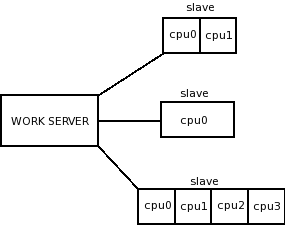
\includegraphics[width=.5\textwidth]{images/workserver_slaves.png}
\caption{Conectando {\it work server} e {\it slaves}.}
\label{fig:serverslaves}
\end{figure}

Não se deve confundir o modelo de computação distribuída da linguagem {\tt pFun} com coleta de lixo paralela. Apesar de enviar computações pela rede, cada {\it slave} em execução realiza sua própria coleta de lixo localmente, de forma totalmente independente. Portanto, a coleta de lixo ocorrerá somente no computador em que a computação estiver executando.

%\section{Sistemas de execução} \label{sec:rts}
%Desenvolvido em \texttt{C}, o sistema de execução (\textit{run-time system}) da linguagem \texttt{pFun} implementa um interpretador de \textit{byte-codes} (pseudo-código gerado pelo compilador) utilizando uma pilha e \textit{stack-frames} para separar chamadas aninhadas de funções. As funcionalidades do interpretador são descritas nas sub-seções seguintes, segundo \cite{ref:pfun}; a exceção é o sistema para gerenciamento automático de memória, que é abordado pela seção \ref{sec:gc}.

%Entre os componentes de uma máquina virtual, está o coletor de lixo, abordado em mais detalhes próximo capítulo \ref{sec:gc}.



\chapter{Gerência automática de memória} \label{sec:memmanag}

\section{Introdução}
Muitas linguagens de programação permitem a alocação dinâmica de blocos de memória cuja existência não está limitada à função criadora. Estes blocos são armazenados no que chamamos de \textit{heap}: porção de memória que armazena dados com escopo indefinido \cite{bib:herlihy:theart}.

Na maioria das linguagens de programação imperativas, a tarefa de alocação e liberação de recursos, enfim, a gerência de memória é atribuída ao programador \cite{bib:lins:gc}. Isto é, após alocar um bloco de memória, o programador decide quando este deve ser liberado, consequentemente, deve-se ter certeza do momento correto para tal. Uma tentativa de acesso, modificação ou liberação de uma área de memória não alocada pode causar interrupção da execução do programa. 
% ou mesmo corromper a execução do sistema operacional (dependendo do sistema). %O trecho de código ~\ref{src:expalloc} mostra como é feita a alocação e liberação da memória na linguagem \texttt{C}.

O termo \textbf{coleta de lixo}, do Inglês \textit{garbage collection}, refere-se a ação de liberar (ou recuperar) automaticamente aqueles objetos (blocos de memória) não mais referenciados pelo programa, deixando espaço livre para futuras alocações \cite{bib:samsom:gengc}. O ponto de partida para a realização da coleta de lixo é chamado conjunto-raiz e, segundo \cite{bib:marcos}, este pode incluir dados globais, dados alocados na pilha de execução e endereços armazenados em registradores. No sistema de execução da linguagem \texttt{pFun}, coleta de lixo é essencial, pois nas linguagens funcionais deve-se especificar funções, sem levar em conta detalhes da execução.

Estudos comprovam que a gerência automática de memória contribui consideravelmente no tempo de execução de um programa, uma vez que o programa deve ser interrompido para realização da coleta de lixo. Richard Jones e Rafael Lins \cite{bib:lins:gc} mencionam que o tempo de execução típico de coletas de lixo pode chegar a 20\% do tempo de execução total do programa. Esta variação dá-se por vários fatores, como a residência máxima da {\it heap}, a estratégia de coleta que está sendo empregada, entre outros.
%como o desempenho da memória {\it cache}, a residência máxima da {\it heap}, a estratégia de coleta que está sendo empregada, entre outros.

%\section{Vantagens da utilização de coleta de lixo} \label{sec:whygc}
%Em linguagens de programação funcionais, a preocupação é com a definição de funções, ou seja, \textbf{o quê} ela deve fazer, não \textbf{como} ela faz. Em programação funcional, o programador não deve se preocupar com a alocação de recursos por parte do programa, o foco deve ser o funcionamento do mesmo.
%Ao programar em uma linguagem que oferece coleta de lixo, o programador concentra seus esforços no conhecimento local da aplicação que está desenvolvendo, alocação e recuperação de memória exigem conhecimento global do programa (AUTHORS HERE). Mais especificamente, programadores não costumam saber que determinada porção de memória está ainda em uso por um trecho de código qualquer; mais difícil é saber o que a aplicação fará com aquela memória em tempo de execução. Ao usar coleta de lixo, o programador é liberado da preocupação com o estado global do programa, podendo se concentrar no mais importante, que é o funcionamento da aplicação.

\section{Ponteiros e alocação dinâmica de memória} \label{sec:ptr}
Na linguagem \texttt{C}, pode-se acessar posições de memória diretamente através de variáveis ou indiretamente, via ponteiros. Variáveis são porções de memória que consistem de um ou mais \textit{bytes} contíguos. Após declarada, toda variável possui um nome, um valor e um endereço de memória; o acesso ao conteúdo de uma variável é feito pelo seu nome. Ponteiros são variáveis que podem armazenar endereços de outras variáveis ou mesmo áreas de memória alocadas. Abaixo, tem-se a declaração de um ponteiro para variáveis do tipo inteiro, em seguida, é mostrado o modo de armazenar o endereço da variável \texttt{number} neste ponteiro. A Figura ~\ref{fig:ptr} é uma representação abstrata de como um ponteiro armazena endereços.

\begin{verbatim}
int number = 5, *ptr;
ptr = &number;
\end{verbatim}

\begin{figure}[htbp]
\centering
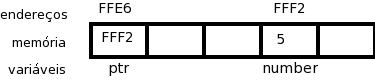
\includegraphics[width=.6\textwidth]{images/pointer.png}
\caption{Como um ponteiro armazena endereços \cite{bib:horton:begc}.}
\label{fig:ptr}
\end{figure}

As declarações de variáveis apresentadas acima são ditas estáticas, pois são definidas em tempo de compilação. O Programa ~\ref{src:expalloc} apresenta um exemplo de alocação dinâmica de memória utilizando a função \texttt{malloc()}, da biblioteca padrão de \texttt{C}. Quando \texttt{malloc()} é utilizada, deve-se especificar a quantidade de \textit{bytes} a serem alocados; a função retorna o endereço do primeiro \textit{byte} da sequência. Como mostrado na linha 12, uma maneira prática de especificar quantos \textit{bytes} devem ser alocados é utilizando o operador unário \texttt{sizeof}, que atua sobre um tipo definido e retorna o número de \textit{bytes} que este ocupa em memória. A estrutura {\tt memblock} ocupa 12 \textit{bytes}. Quando {\tt bp} não for mais utilizada, esta deve ser liberada manualmente utilizando a função {\tt free()} (linha 14).

\lstinputlisting[language=C, label=src:expalloc,
								 caption=Alocando memória explicitamente.]
								 {codes/explicit_alloc.c}


\section{Objetos inalcançáveis} \label{sec:unreach}
Objetos alocados dinamicamente podem se tornar inalcançáveis, como mostra o Programa \ref{src:unreach}, escrito na linguagem \texttt{C}. Neste caso, tem-se a alocação de um bloco de memória apontado por \texttt{x}, em seguida, a porção de memória referenciada por \texttt{x} é modificada. Entretanto, a linha 5 aloca uma nova área de memória fazendo com que \texttt{x} aponte para esta, então, a memória contendo os valores
\begin{center} $a=30$ e $b=87.2$ \end{center}
não está mais acessível, pois nenhuma outra variável ponteiro armazena seu endereço. Esta porção de memória inacessível é chamada lixo, e será desalocada apenas quando o programa encerrar.

\lstinputlisting[language=C, label=src:unreach,
								 caption=Tornando uma área de memória inalcançável.]
								 {codes/unreachable.c}

%Deste modo, é possível fazer um programa cuja finalidade é consumir recursos do sistema sem liberá-los...

%A typical approach to garbage collection is therefore to identify all reachable objects and reclaim any previously allocated memory that the reachable objects do not occupy. A typical garbage collector may identify reachable objects by tracing objects pointed to from a root, tracing objects pointed to from those reachable objects, and so on until all the referenced or pointed to objects are found and are retained. Thus the last objects found will have no pointers to other untraced objects. In this way unreachable objects are in effect discarded and their memory space becomes free for alternative use.

%\section{Sistemas de execução} \label{sec:rts}
%Sistema que interpreta código escrito em determinada linguagem (REFORMULAR).

%\subsection{Ambientes baseados em pilhas}
%Em linguagens que permitam chamadas recursivas de procedimentos/funções, nas quais variáveis locais recebam novas posições a cada invocação, os registros de ativação (O Q É UM REGISTRO DE ATIVAÇÃO???) não podem ser alocados estaticamente \cite{bib:louden}. Em vez disso, a cada novo registro, este deve ser alocado no topo de uma pilha. Assim, cada função pode manter vários registros distintos na pilha ao mesmo tempo, cada um deles representando uma chamada diferente. Deve-se guardar informações adicionais que permitam preservar a sequência de chamadas de funções.

%\subsection{Sistemas totalmente dinâmicos}
%Segundo Louden \cite{bib:louden} princípio essencial no projeto de uma linguagem funcional é fazer com que as funções sejam o mais gerais quanto possível, ou seja, funções podem ser definidas com escopo local, passadas como argumentos e retornadas como resultado. Portanto, para esta classe de linguagens, um sistema de execução baseado em pilhas é inadequado, sendo necessário uma forma mais genérica de ambiente. Estes são conhecidos como sitemas de execução totalmente dinâmicos, pois descartam os registros de ativação apenas quando estes não forem mais referenciados, visto que devem ser liberados dinamicamente em instantes arbitrários durante a execução.

%Sistemas de execução dinâmicos são mais complexos que sistemas baseados em pilhas, pois exigem o acompanhamento das referências durante a execução e gerência automática de memória.


\section{Características de sistemas para coleta de lixo}
A primeira linguagem a liberar memória automaticamente foi \texttt{Lisp} em 1958. Atualmente, muitas linguagens de alto nível oferecem coleta de lixo sem a participação ou mesmo sem o conhecimento do programador. Algumas implementações importantes incluem \texttt{Java}, \texttt{Perl}, \texttt{Haskell}, \texttt{Python}, \texttt{Prolog} e \texttt{Smalltalk}. Aho \cite{bib:aho:comp} cita algumas considerações no projeto de um sistema coletor de lixo:

\begin{itemize}
\item Tempo de execução: é importante que o tempo de execução da coleta de lixo não aumente significativamente o tempo total de execução da aplicação. Uma vez que o coletor deve manipular muitos dados, a eficiência no acesso a memória do sistema computacional é bastante relevante;

\item Aproveitamento de espaço: é importante que a coleta de lixo evite fragmentação e use com eficiência a memória disponível;

\item Tempos de pausa: estratégias \textit{stop-the-world}, onde sistema de execução da linguagem interrompe a execução do programa principal em favor da realização da coleta de lixo, são conhecidas por causarem pausas repentinas no programa. Consequentemente, é importante que os tempos de pausa sejam minimizados;

\item Localidade do programa: não se pode avaliar um algoritmo coletor de lixo somente pelo tempo de execução. Coletores de lixo reposicionam dados, influenciando na localidade dos objetos do programa escrito pelo usuário da linguagem e nos dados da memória cache.
\end{itemize}


\section{Estratégias para coleta de lixo aplicadas na \texttt{pFun}} \label{sec:gcpfun}
A linguagem \texttt{pFun} possui duas estratégias \textit{stop-the-world} de coleta de lixo implementadas: coleta de cópia de dois espaços \cite{bib:dubois:pfun} e coleta baseada em gerações utilizando o algoritmo \textit{mark-and-compact} para coleta da geração antiga \cite{bib:beloni}. Estas estratégias são detalhadas nas próximas seções.

\subsection{Coleta de cópia de dois espaços} \label{sec:twospace}
Este algoritmo divide a \textit{heap} em duas regiões, uma ativa (onde os objetos novos serão alocados) e outra inativa, ou auxiliar \cite{bib:samsom:gengc}. Quando a coleta é iniciada, a porção ativa atua como uma região de origem, onde busca-se os objetos referenciados diretamente pelo conjunto-raiz do programa \texttt{pFun} (pilha de execução e tarefas remotas), então apenas os objetos vivos são copiados para a porção inativa (região de destino) da {\it heap}.

O fluxograma da Figura \ref{fig:copyflow} apresenta, resumidamente, o funcionamento da coleta de cópia de dois espaços. Primeiramente, percorre-se o conjunto-raiz do programa, copiando suas referências diretas para a região de destino através de um processo chamado {\it evacuate}.

Neste fluxograma, as variáveis {\tt tospace} e {\tt tstop} indicam, respectivamente, o início da região de destino e o topo desta região, que vai sendo incrementado a medida que novos objetos vão sendo copiados. O passo seguinte é efetuar uma busca em extensão por todos os objetos já copiados ({\it scavenge}), visando copiar também suas referências ou atualizá-las, no caso de já estarem na região de destino. Para tal, uma variável auxiliar {\tt walk} começa a percorrer os objetos já copiados a partir do início região de destino, se o objeto possi referências a outros objetos, deve-se aplicar um {\it evacuate} em cada uma dessas referências. Por fim, ocorre um teste para verificar se {\tt walk} percorreu todos objetos da região de destino; atualiza-se o novo topo da {\it heap}; e a região inativa torna-se ativa para a próxima coleta e vice-versa.

\begin{figure}[h]
\centering
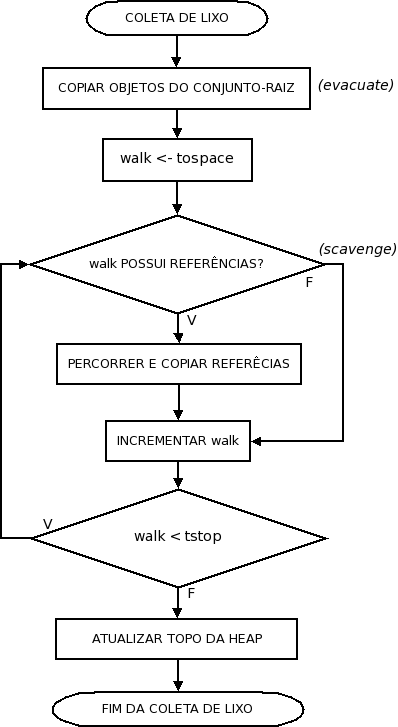
\includegraphics[width=.45\textwidth]{images/copy_flow.png}
\caption{Fluxograma referente a coleta de cópia de dois espaços.}
\label{fig:copyflow}
\end{figure}

%\lstinputlisting[language=C, label=src:twospace,
%								 caption=Implementação da coleta de cópia de dois espaços.]
%								 {codes/twospace.c}

A Figura \ref{fig:twospacefull} mostra o estado da região ativa da \textit{heap} quando está no limite da capacidade, percebe-se que muitos objetos, como $O_{16}, O_{11}$ e $O_{12}$ não estão acessíveis através do conjunto-raiz ou mesmo indiretamente por outro objeto, portanto não são considerados vivos. A Figura \ref{fig:twospacecol} ilustra os objetos sobreviventes que foram copiados para a região inativa. Percebe-se que o conjunto-raiz agora aponta para a região antes inativa, que se tornou ativa ao final do processo.

\begin{figure}[h]
\centering
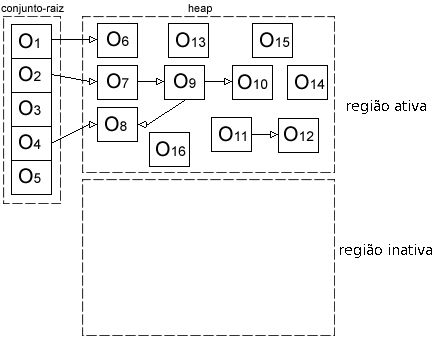
\includegraphics[scale=.55]{images/twospace_full.png}
\caption{Região ativa lotada: antes da coleta de lixo \cite{bib:marcos}.}
\label{fig:twospacefull}
\end{figure}

Segundo \cite{bib:marcos}, a coleta de cópia é uma boa opção quanto a velocidade em tempo de execução, mas é preciso que a disponibilidade de memória não seja escassa, visto que esta aproveita apenas metade da memória disponível. %Apesar de não ser o mais indicado, 
A coleta de cópia foi escolhida para ser paralelizada neste projeto, principalmente por sua relativa simplicidade da implementação sequencial e por ser muito utilizada na recuperação de memória das gerações jovens em um esquema de gerações.

%Outra característica importante deste algoritmo é que o sistema de execução da linguagem interrompe a execução do programa principal em favor da realização da coleta de lixo de dois espaços.

\begin{figure}[h]
\centering
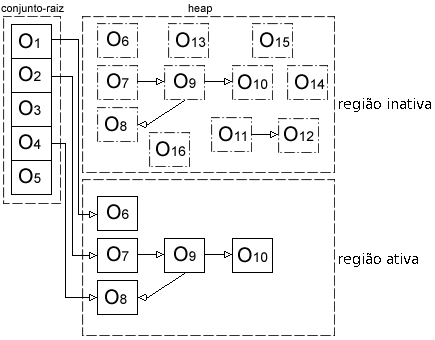
\includegraphics[scale=.55]{images/twospace_collected.png}
\caption{Nova região ativa contendo os sobreviventes \cite{bib:marcos}.}
\label{fig:twospacecol}
\end{figure}

\subsection{Coleta baseada em gerações utilizando \textit{mark-and-compact}} \label{sec:gen}
De acordo com os Jones e Lins \cite{bib:lins:gc}, a maioria dos objetos alocados tornam-se inalcançáveis com pouco tempo de vida, o que chamamos de {\bf hipótese de gerações}. A coleta de lixo baseada em gerações faz a recuperação da memória de forma mais eficiente e com menos interrupções, pois concentra seus esforços em coletar aqueles objetos mais propícios a se tornarem lixo: os mais jovens.

O algoritmo de gerações separa os objetos por tempo de vida, formando as gerações, de modo que os espaços de alocação para as gerações jovens sejam menores se comparados a área reservada para as gerações antigas. Diferentes gerações são coletadas em diferentes frequências, onde as gerações mais jovens são coletadas mais frequentemente (coletas minoritárias) e as gerações mais antigas são coletadas com menor frequência (coletas majoritárias) \cite{bib:lins:gc}.

\begin{figure}[h]
\centering
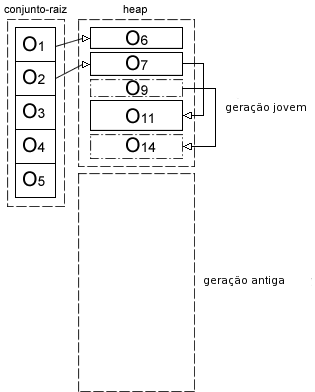
\includegraphics[scale=.55]{images/gen_young.png}
\caption{Geração jovem lotada \cite{bib:marcos}.}
\label{fig:genyoung}
\end{figure}

No esquema com apenas duas gerações, os objetos são alocados primeiramente na geração jovem e, quando esta estiver lotada, os objetos vivos ($O_6$, $O_7$ e $O_{11}$ da Figura \ref{fig:genyoung}) são promovidos para a geração mais antiga. O processo de promoção nada mais é do que uma cópia (ao estilo cópia de dois espaços) de objetos da geração jovem para a geração antiga, que vai acumulando os sobreviventes de várias coletas à geração jovem, como mostra a Figura \ref{fig:genpromot}. A coleta da geração antiga ocorre quando esta estiver lotada, utilizando o algoritmo \textit{mark-and-compact}. O fluxograma da Figura \ref{fig:markcompflow} é um resumo deste algoritmo.%; o mesmo é dividido em três fases:  %sua implementação é mostrada no Programa \ref{src:markcomp}.


\begin{figure}[h]
\centering
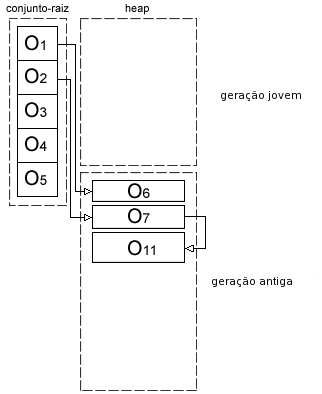
\includegraphics[scale=.55]{images/gen_promot.png}
\caption{Objetos sobreviventes promovidos a geração antiga \cite{bib:marcos}.}
\label{fig:genpromot}
\end{figure}

\pagebreak

%\begin{itemize}
%\item Marcar objetos alcançáveis pelo programa e suas referências recursivamente a partir do conjunto-raiz;
%\item Realocar os objetos de forma a compactar a \textit{heap} e liberar espaço para futuras alocações;
%\item Atualizar as referências dos objetos sobreviventes;
%\end{itemize}

%\lstinputlisting[language=C, label=src:markcomp,
%								 caption=Compactação da geração antiga.]
%								 {codes/mark-and-compact.c}

\begin{figure}[h]
\centering
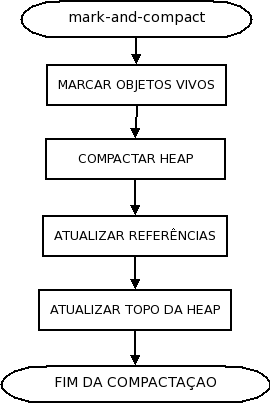
\includegraphics[width=.40\textwidth]{images/mark-and-compact_flow.png}
\caption{Fluxograma referente ao algoritmo {\it mark-and-compact}.}
\label{fig:markcompflow}
\end{figure}

O algoritmo {\it mark-and-compact} possui complexidade computacional $O(n)$, pois cada uma das fases percorre, no pior caso, todos os elementos da geração antiga. Na coleta da geração antiga, este algoritmo exige quantidade de memória do tamanho da área a ser coletada, já que deve-se armazenar os novos endereços de memória dos objetos realocados.


%\chapter{Processamento paralelo revisitado} \label{sec:parproc}
\chapter{Programação de arquiteturas paralelas} \label{sec:parproc}

\section{Introdução}
Um programa paralelo, ou concorrente, consiste basicamente de dois ou mais fluxos de execução trabalhando juntos para resolver um problema. Os fluxos de execução podem trocar informações através de variáveis compartilhadas (seção \ref{sec:sharedmem}) ou envio de mensagens pela rede.

Programas paralelos podem aumentar o desempenho em relação a sua versão sequencial somente se executarem sobre uma arquitetura com vários processadores. Infelizmente, o aumento do número de unidades de processamento acaba por complicar o desenvolvimento de aplicações que tiram proveito dessas arquiteturas, tanto no gerenciamento da comunicação entre os fluxos de execução, mas sobretudo no particionamento dos problemas em várias unidades ativas, como aborda a seção \ref{sec:workdistrib}. %Dependendo da natureza do programa e do tipo de arquitetura paralela escolhida, o {\it overhead} acrescentado em sua paralelização acaba tornando-o mais lento, pois utiliza-se mais memória para o gerenciamento

\section{Arquiteturas de memória compartilhada} \label{sec:sharedmem}
Neste tipo de arquitetura, múltiplos nodos de processamento têm acesso a uma memória comum (compartilhada) por meio de um barramento de interconexão implícito, como mostra a Figura \ref{fig:smp}, por este motivo, são também conhecidos por multiprocessadores. Adenauer Yamin \cite{bib:adenauer} cita alguns aspectos positivos do uso de arquiteturas de memória compartilhada:

\begin{itemize}
\item A localidade do processador é abstraída nestas arquiteturas: a comunicação é feita através de leitura e escrita em variáveis compartilhadas com alto desempenho;

\item Semelhante às arquiteturas de único processador: ambiente de programação e sistema operacional operam de forma semelhante nas arquiteturas multiprocessadas e de único processador;

\item Compartilhamento de recursos: a memória comum facilita o compartilhamento de dados, recursos de entrada/saída e memória virtual.
\end{itemize}

\begin{figure}[htbp]
\centering
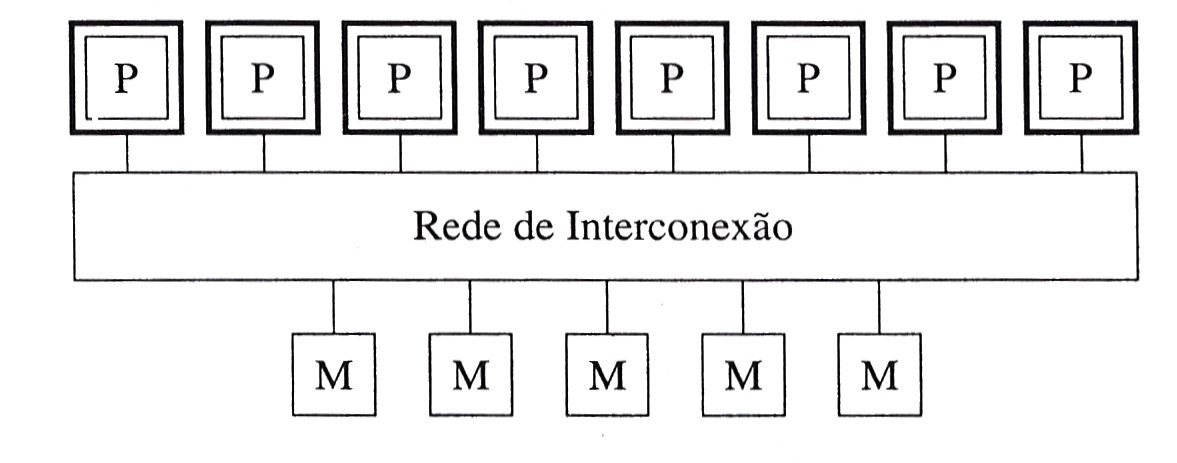
\includegraphics[scale=1]{images/smp1.jpg}
\caption{Arquitetura genérica de processadores com memória compartilhada \cite{bib:crad}.}
\label{fig:smp}
\end{figure}

Existem diversas formas de interligar processadores e memórias na definição de uma arquitetura paralela. Cada estratégia de interconexão tem implicações diretas em aspectos operacionais: desempenho, escalabilidade, custo de fabricação, entre outros. %As subseções a seguir, baseadas no texto de César De Rose \cite{bib:crad}, apresentam três arquiteturas de processadores de memória compartilhada.

%\subsection{Acesso uniforme à memória}
%Nessas arquiteturas, a memória é centralizada, encontrando-se à mesma distância de todos os processadores, consequentemente a latência de acesso à memória é a mesma (uniforme) para todos os processadores do sistema, como mostra a Figura \ref{fig:uma}.

%\begin{figure}[htbp]
%\centering
%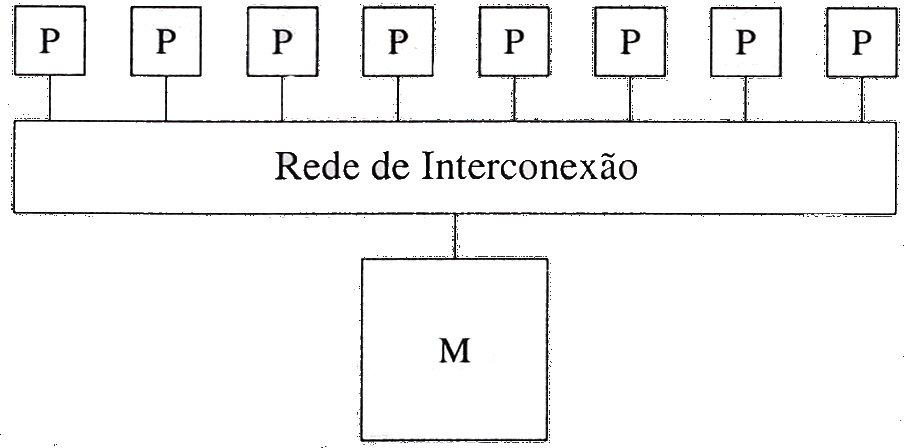
\includegraphics[scale=1.3]{images/uma.jpg}
%\caption{Arquitetura de processadores com acesso uniforme à memória \cite{bib:crad}.}
%\label{fig:uma}
%\end{figure}

%\subsection{Acesso não uniforme à memória}
%A memória é distribuída, implementada como múltiplos módulos que são associados cada um a seu respectivo processador. Entretanto o espaço de endereçamento é único e qualquer processador pode endereçar toda memória do sistema. Se o endereço solicitado pelo processador encontrar-se no módulo de memória local, o tempo de acesso será menor se comparado ao tempo de acesso à memória de outro processador. Por isso, a latência de acesso à memória não é uniforme, como mostra a Figura \ref{fig:numa}.

%\begin{figure}[htbp]
%\centering
%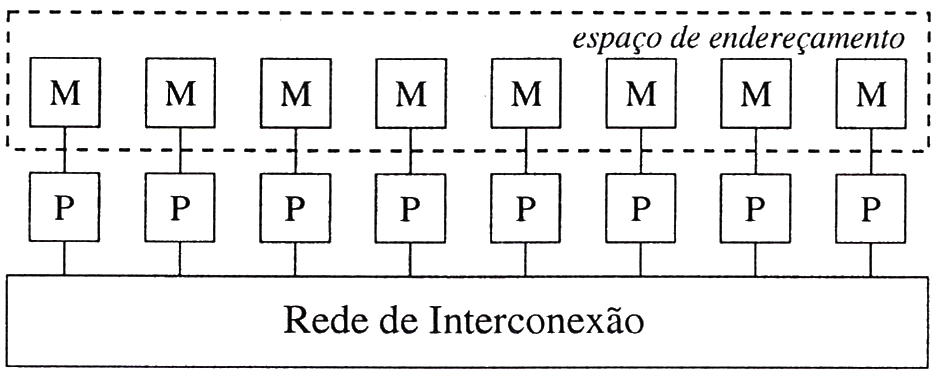
\includegraphics[scale=1.3]{images/numa.jpg}
%\caption{Arquitetura de processadores com acesso não uniforme à memória \cite{bib:crad}.}
%\label{fig:numa}
%\end{figure}

\subsection{Processadores multicore}
Esta arquitetura se popularizou devido à sua adoção nos computadores pessoais comerciais. É dita simétrica porque todos processadores têm igual acesso ao barramento e à memória. Na Figura \ref{fig:smp2}, percebe-se que o barramento que dá acesso à memória é único, ou seja, ocorre um chaveamento que decide qual processador (P/C) acessará ao módulo de memória (MC) em um dado instante.


\begin{figure}[htbp]
\centering
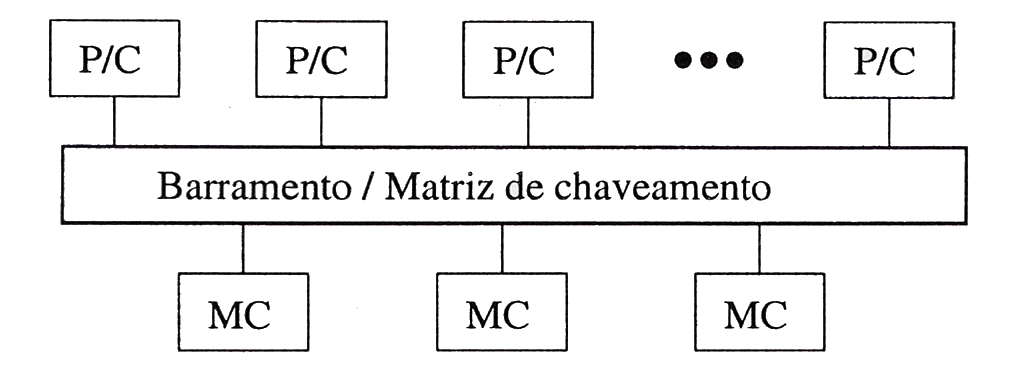
\includegraphics[scale=1.1]{images/smp2.jpg}
\caption{Processadores multicore comerciais \cite{bib:crad}.}
\label{fig:smp2}
\end{figure}

Um processador multicore combina dois ou mais núcleos de processamento independentes em um circuito integrado. Os núcleos de processamento podem ou não compartilhar a memória cache, compartilham as interconexões com o restante do sistema e implementam as mesmas otimizações existentes em processadores simples, como {\it pipelining}, {\it multi-threading}, etc. É importante observar, ainda na Figura \ref{fig:smp2}, que a memória cache está representada juntamente com o respectivo processador, antes do barramento de interconexão, visto que, em uma arquitetura com muitos processadores, várias tentativas de acesso à memória principal podem ocasionar um gargalo.

\subsection{Memórias cache e coerência} \label{sec:cache}
Nas arquiteturas modernas, acesso a dados na memória principal pode levar centenas de ciclos, fazendo com que processadores percam muito tempo apenas esperando por requisições à memória principal \cite{bib:herlihy:theart}. Este gargalo é reduzido com o uso de memórias cache: pequenas memórias que situam-se logicamente entre o processador e a memória principal, portanto mais rápidas. Quando um processador precisa de um valor de um certo endereço de memória, primeiramente este deve verificar se o valor já está na cache. Se encontrado, não será necessário acessar a memória principal, neste caso tem-se o chamado cache {\it hit}; caso contrário, tem-se um cache {\it miss} e o valor terá de ser buscado na memória principal.

Segundo \cite{bib:herlihy:theart}, caches demonstram-se efetivas devido ao alto grau de localidade que apresentam os processadores: uma vez que um valor foi modificado na memória, é bastante provável que o respectivo endereço seja requisitado brevemente. Além disso, sabe-se que os endereços próximos àquele modificado também possuem grande probabilidade de acesso (no uso de {\it arrays}, por exemplo), por isso, as memórias cache não só armazenam o conteúdo do endereço de memória requisitado, mas também dos seus vizinhos. Memórias cache são mais caras de produzir, portanto muito menores que as memórias principais, consequentemente apenas uma pequena fração da memória principal poderá estar em cache.

%\subsubsection{Coerência}
Em um sistema multiprocessado, contenções de memória ocorrem quando processadores leem ou modificam endereços de memória situados na cache de outro processador. Se dois processadores apenas fazem a leitura de uma área de memória, ambos podem armazenar este dado em suas caches. Entretanto, quando um processador tenta atualizar o conteúdo de um endereço armazenado na sua respectiva cache, uma eventual leitura de outro processador ao mesmo endereço em cache deve ser invalidada. Este é o chamado problema de coerência de cache: deve haver uma consistência dos dados armazenados em diferentes caches que façam referência à uma memória comum, como mostra a Figura \ref{fig:cache}. Existem vários protocolos para tratar este problema, mas o importante é projetar o sistema de forma a evitar contenções geradas por dados espalhados em múltiplas caches.
% Herlihy e Shavit comentam que existem vários protocolos para tratar este problema, e afirmam que o mais importante é projetar o sistema de forma a evitar contenções geradas por dados espalhados em múltiplas caches.

\begin{figure}[h]
\centering
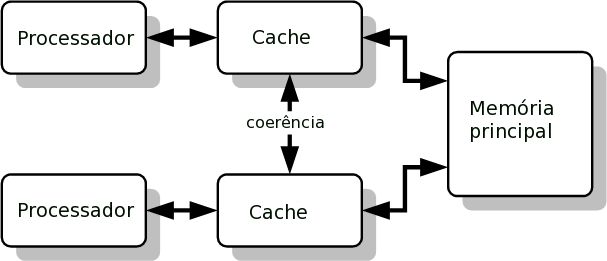
\includegraphics[scale=.86]{images/Cache_Coherency.png}
\caption{Coerência de cache.}
\label{fig:cache}
\end{figure}


\section{\textit{Threads}} \label{sec:threads}
Chama-se \textit{thread} cada um dos fluxos de execução em que pode-se dividir um programa. Diferentes \textit{threads} criadas por um mesmo processo\footnote{Instância de um programa em execução.} compartilham recursos através de variáveis globais. O uso de \textit{threads} é um dos mecanismos empregados para tirar proveito do paralelismo inerente a determinados problemas, mas cabe ao programador saber organizar seu programa para que este obtenha o melhor desempenho possível. Existem muitos problemas que possuem partes que não são facilmente paralelizáveis devido ao acesso concorrente aos dados e a necessidade de coordernação de \textit{threads}.

O autor Mark Mitchell \cite{bib:advlinprog} explica que, no padrão POSIX, {\it threads} são escalonadas de forma assíncrona pelo núcleo do sistema operacional, de modo que a ordem de execução das instruções é imprevisível. Cada {\it thread} pode criar outras {\it threads} e cada uma delas, apesar de executarem no mesmo processo, podem estar em diferentes pontos do programa a qualquer momento. Novas {\it threads} são criadas compartilhando o mesmo espaço de memória, descritores de arquivos e outros recursos do sistema. Portanto, pode-se fazer a intercomunicação entre {\it threads} utilizando variáveis globais. Todavia, {\it threads} possuem sua própria pilha de execução, possibilitando a execução e retorno de funções da mesma maneira que qualquer programa.

Se a arquitetura não dispõe de vários processadores, um programa {\it multi-thread}\footnote{Processos com mais de uma \textit{thread} em execução.} executará virtualmente de forma paralela através da multiplexação de tempo por parte do sistema operacional: serão oferecidas várias fatias de tempo para execução de cada \textit{thread}. Em arquiteturas multicore, diferentes \textit{threads} podem executar, literalmente ao mesmo tempo, em diferentes processadores, desde que estejam disponíveis.

\section{Sincronização e seções críticas}
Segundo \cite{bib:advlinprog}, o maior benefício dos programas {\it multi-thread} é também o maior causador de erros: dados compartilhados que podem ser acessados ao mesmo tempo. Se uma {\it thread} está atualizando uma estrutura de dados no exato momento que outra {\it thread} acessa a mesma estrutura, um erro poderá ocorrer. Estas situações são chamadas condições de corrida (do Inglês, {\it race conditions}): quando uma {\it thread} concorre com outra no acesso ou modificação da mesma área de memória.

\subsection{Condições de corrida}
Para exemplificar o problema gerado por uma condição de corrida, os autores \cite{bib:advlinprog} utilizam uma fila de tarefas {\tt tasks}, que é representada por uma lista encadeada do tipo {\tt struct task}, como mostra o Programa \ref{src:taskque}. Na repetição das linhas 12 a 18, primeiramente ocorre a verificação se a fila ainda possui elementos, depois o primeiro elemento é retirado e a tarefa correspondente é executada, e assim por diante até o ponteiro {\tt tasks} se tornar nulo.

Supondo que duas {\it threads} terminem o procedimento {\tt execute()} ao mesmo tempo, deixando apenas um elemento na fila de tarefas. Uma {\it thread (A)} entra na repetição da linha 12 e obtém o primeiro elemento da fila. Neste mesmo período, outra {\it thread (B)} é escalonada pelo sistema operacional, procede a execução da última tarefa e termina a função. Quando {\it thread (A)} retornar, ao executar a linha 15 -- tentativa de acesso à variável membro {\tt tasks->next} -- causará um acesso indevido à memória. Esta condição de corrida não vai ocorrer todas as vezes que o programa for executado, mas pode ocorrer e deve ser evitada. \vskip 10pt

\lstinputlisting[language=C, label=src:taskque,
								 caption=Função de {\it thread} para executar tarefas de uma lista encadeada.]
								 {codes/task_queue.c}

%USE Adv. lINUX  prog book examples
% see chap 4.4 adv linux prog

\subsection{\textit{Mutexes}}
Uma das maneiras de evitar o problema abordado na seção anterior é a demarcação da seção crítica do programa com exclusão mútua, ou seja, determinado trecho de código deve ser executado atomicamente: uma operação indivisível e ininterrupta. Uma vez que iniciam, operações atômicas não são interrompidas até que terminem. POSIX {\it threads} oferece exclusão mútua através dos {\it mutexes (MUtual EXclusion locks)}.

No problema do Programa \ref{src:taskque}, deve-se fazer com que cada {\it thread} possa acessar a fila de tarefas por vez -- guardar o primeiro elemento e removê-lo da fila  -- só então executar a tarefa. O Programa \ref{src:taskmutex} \cite{bib:advlinprog} mostra uma fila de tarefas protegida contra vários acessos simultâneos de {\it threads}. 

De acordo com o Programa \ref{src:taskmutex}, um {\it mutex} é criado declarando-se uma variável do tipo {\tt pthread\_mutex\_t}, como mostra a linha 8, onde o mesmo também é inicializado. Um {\it mutex} é um tipo de ``tranca'' que apenas uma {\it thread} pode trancar por vez. Ao entrar na seção crítica, uma {\it thread (A)} tranca o {\it mutex} (linha 15). Outras {\it threads} que tentarem executar a mesma linha ficarão bloqueadas até que a {\it thread (A)} libere o {\it mutex} (linha 22). Só então uma das outras {\it threads} poderá trancar o {\it mutex} para executar a seção crítica.

É importante observar que, apenas pelo fato de uma {\it thread} liberar o {\it mutex}, não implica que outra {\it thread} terá acesso à seção crítica imediatamente. O que determina o momento em que {\it threads} são executadas é o escalonador do sistema operacional, levando em consideração o número de processadores disponíveis, sua carga, entre outros.

\lstinputlisting[language=C, label=src:taskmutex,
								 caption=Fila de tarefas com acesso limitado a uma {\it thread} por vez.]
								 {codes/task_queue_mutex.c}

Seções críticas são determindadas pelo programador, ficando compreendidas entre chamadas às funções {\tt pthread\_mutex\_lock()}, para trancar o {\it mutex} e {\tt pthread\_mutex\_unlock()}, para destrancá-lo. Todos acessos à fila compartilhada {\tt tasks} devem ser feitos dentro da seção crítica. Uma tarefa ({\tt next\_task}) é acessada fora desta região depois de ter sido removida da fila, portanto, não mais acessível a outras {\it threads}.

\section{Instrução \textit{compare-and-swap}}
Na coleta de lixo, o processo de tranferência dos objetos vivos de uma região para outra permite que mais de uma {\it thread} referencie o mesmo objeto, mas apenas uma {\it thread} deve copiá-lo, portanto é preciso verificar se o objeto em questão já foi copiado. Para tal, esta implementação faz uso da instrução {\it compare-and-swap} (CAS), conhecida como {\it cmpxchg (compare-and-exchange)} na arquitetura Intel x86. Esta instrução faz, atomicamente, a comparação e, se necessário, a atualização de uma posição de memória.

De acordo com o Programa \ref{src:cas}, a instrução CAS (rotina {\tt cmpxchg} da linha 9) recebe três argumentos: uma referência a uma posição de memória {\tt mem}, o valor que se espera encontrar {\tt old} no conteúdo de {\tt mem} e um novo valor {\tt new} a ser atualizado em {\tt mem}. Se o valor contido em {\tt old} for igual ao conteúdo referenciado por {\tt mem}, CAS procede a cópia de {\tt new} em {\tt mem}. Caso contrário, {\tt old} diferente do valor referencioado por {\tt mem}, nada é feito.

O valor {\tt res} retornado pela rotina {\tt cmpxchg} contém o valor inicial apontado por {\tt mem} e, ao ser comparado ao valor {\tt old}, indica o sucesso ou falha da operação. Se o Programa \ref{src:cas} executar a linha 10, significa que a operação CAS foi realizada com sucesso, sendo que {\tt mem} agora referencia o mesmo valor de {\tt new}.

\lstinputlisting[language=C, label=src:cas,
								 caption=Funcionamento da instrução CAS.]
								 {codes/cas.c}

A partir da linha 15 (função {\tt main()}), o Programa \ref{src:cas} faz com que {\tt mem} referencie uma área de memória contendo o valor 777. Após, duas {\it threads} são criadas, passando como último argumento, um valor qualquer, que será atribuído a variável {\tt old} na função da thread (linha 6). Ao executar {\tt cmpxchg()}, a {\it thread} em que o teste {\tt old == *mem} for verdadeiro terá sucesso, copiando {\tt old} para {\tt *mem}. A seguir, tem-se um exemplo de saída gerada pelo Programa \ref{src:cas}, onde são mostrados também os valores das variáveis envolvidas na operação CAS:
\begin{verbatim}
thread 16386 mem: 777, old: 555, new: 999
thread 16386: CAS failed...
thread 16386 mem: 777, old: 555, new: 999, res: 777

thread 32771 mem: 777, old: 777, new: 999
thread 32771: CAS sucess!
thread 32771 mem: 999, old: 777, new: 999, res: 777
\end{verbatim}

Seguindo a estrutura proposta por Flood e Detlefs \cite{bib:flood:pargc}, CAS é utilizada na alocação do espaço de memória para cada objeto na região de destino. Se este já possui uma cópia na referida região, CAS falhará, a cópia não será efetuada e o endereço do correspondente objeto já copiado para a região de destino deve ser referenciado pelo objeto em questão. CAS sucede quando o objeto ainda não possui cópia na região de destino, procedendo a alocação e sinalização do novo endereço do objeto. A seção \ref{sec:cas} mostra como CAS é aplicada neste projeto.


\section{Distribuição de tarefas} \label{sec:workdistrib}
Sabe-se que alguns problemas podem ser facilmente projetados para execução em paralelo. % através de \textit{threads}. 
Herlihy \cite{bib:herlihy:theart} cita o exemplo de requisições que chegam em um servidor \textit{web}: a cada requisição, o servidor pode apenas criar uma \textit{thread} para tratá-la enquanto continua esperando por outras requisições.

Por outro lado, existem problemas que são inerentemente paralelizáveis, mas não é simples tirar vantagem deste paralelismo. No caso da multiplicação de matrizes, onde
\begin{center} $c_{ij}=\sum\limits_{k=0}^{n-1}a_{ki}×b_{jk}$ \end{center}
se cada $c_{ij}$ for computado por uma nova \textit{thread}, a princípio parece uma boa solução: o programa é altamente paralelo e não exige sincronização de {\it threads}. Mas, segundo Herlihy e Shavit \cite{bib:herlihy:theart}, deste modo o programa apresentará bom desempenho apenas para pequenas matrizes, já para grandes matrizes, a eficiência será comprometida. Visto que criar, escalonar e destruir \textit{threads} possui considerável custo computacional, despachar várias \textit{threads} com curto tempo de vida (poucas computações) é uma maneira bastante ineficiente de projetar uma computação paralela. Uma maneira mais eficiente de organizar tais programas é mantendo um conjunto de {\it threads} ({\it thread pool}) de longa duração, onde cada {\it thread} busca tarefas para executar até que não existam mais tarefas. 


%\section{Lei de Amdahl}
%Segundo Maurice Herlihy \cite{bib:herlihy:theart}, o ideal seria que, aumentando em $n$ o número de processadores de uma arquitetura, o poder de computação deveria aumentar, proporcionalmente, $n$ vezes. Entretanto, isto não acontece, pois aplicações computacionais não são efetivamente paralelizáveis sem o custo adicional com a comunicação entre os processadores envolvidos e a coordernação de {\it threads}.

%A lei de Amdahl enuncia que o ganho máximo de uma aplicação paralela é limitado pelo quanto desta tarefa tiver de ser executada sequencialmente. {\it Speedup} é a taxa de tempo que uma tarefa demora para executar em apenas um processador versus o tempo de execução da mesma tarefa em $n$ processadores. Esta lei determina o máximo {\it speedup} $S$ que se pode conseguir com $n$ processadores trabalhando juntos, sendo $p$ a porção da tarefa que pode ser executada em paralelo.

%Assumindo que uma tarefa demora $T_s$ unidades de tempo em um único processador; com $n$ processadores, a parte paralela executa em $p/n$ e a parte sequencial leva $T_s-p$ unidades de tempo, o tempo de computação em paralelo segue a fórmula:
%$$T_p=T_s-p+\dfrac{p}{n}$$
%e, segundo a lei de Amdahl, o {\it speedup}:
%$$S=\dfrac{T_s}{T_p}$$


\chapter{Estrutura do sistema para coleta de lixo paralela} \label{ch:paralgo}

\section{Introdução}
A crescente popularização dos computadores pessoais multicore oferece grande poder computacional que, muitas vezes, acaba não sendo aproveitado, tanto pelo usuário final como por parte dos programadores. As linguagens de programação modernas cada vez mais oferecem recursos de forma transparente aos desenvolvedores, entre eles está o gerenciamento automático de memória.

No caso das linguagens funcionais, onde a preocupação é com a definição matemática das funções, coleta de lixo é uma exigência: o programador não deve ter o conhecimento do uso da memória por parte de seu programa, muito menos o número de núcleos de processamento disponíveis. O que espera-se de uma boa linguagem de programação funcional é que esta aproveite ao máximo os recursos computacionais sem exigir do programador conhecimento sobre o {\it hardware} disponível. %RECURSOS DIDPONÍVEIS

Segundo \cite{bib:lins:gc}, um sistema para coleta de lixo deve obedecer as seguintes propriedades:
\begin{itemize} % SEE PAGE 304 RAFAEL LINS
\item Abrangência: um coletor de lixo deve ser capaz de coletar todos objetos vivos e descartar o lixo;

\item Corretude: apenas objetos considerados lixo devem ser descartados;

\item Eficácia: os {\it overheads} de tempo gasto e espaço ocupado em memória devem ser aceitáveis.
\end{itemize}

Sabe-se que uma estratégia baseada em gerações utiliza a coleta de cópia na promoção dos objetos vivos, onde a região de origem é a própria geração jovem, enquanto a geração antiga assume o papel de região de destino (seção \ref{sec:gen}). Uma vez que a coleta de cópia de dois espaços é um dos componentes da coleta baseada em gerações e que recuperações de memória na geração jovem são realizadas com muito mais frequência, é conveniente que as coletas minoritárias sejam otimizadas. Para que programas {\tt pFun} possam tirar proveito das arquiteturas multicore, cada vez mais acessíveis no mercado, este projeto visa a paralelização de uma estratégia de coleta de lixo, a coleta de cópia de dois espaços. Tem-se por objetivo diminuir o gargalo da coleta de lixo e, por consequência, reduzir o tempo total de execução de programas na máquina virtual {\tt pFun}, além de contribuir com futuros trabalhos sobre a paralelização da coleta de lixo baseada em gerações. %, numa proporção ASSUSTADORAMENTE ESMAGADORA

%Para que programas {\tt pFun} possam tirar proveito das arquiteturas multicore, cada vez mais acessíveis no mercado, este projeto visa a paralelização de uma estratégia de coleta de lixo, a coleta de cópia de dois espaços. Pretende-se verificar sua viabilidade e benefícios em relação às implementações sequenciais. Tem-se por objetivo diminuir o gargalo da coleta de lixo e, por consequência, reduzir o tempo total de execução de programas na máquina virtual {\tt pFun}.

\section{Paralelização da coleta de lixo}
Com base na proposta de Christine Flood e David Detlefs \cite{bib:flood:pargc}, as próximas seções apresentam a estrutura do sistema para coleta de lixo a ser utilizada neste projeto. É importante ressaltar que esta implementação não constitui uma abordagem prática, mas sim um ensaio, servindo apenas como um modelo para estudos relacionados a coleta de lixo paralela, seus desafios e comportamento, não estando completamente funcional. %WHAT A MESS!

\begin{figure}[h]
\centering
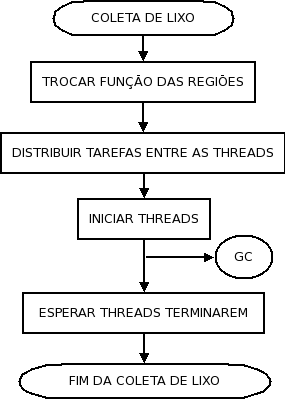
\includegraphics[width=0.4\textwidth]{images/gc_flow1.png}
\caption{Fluxograma do algoritmo para coleta de lixo paralela.}
\label{fig:flow1}
\end{figure}

A Figura \ref{fig:flow1} é um fluxograma que representa a coleta de cópia de dois espaços, juntamente com o mecanismo de paralelização. Com base no conteúdo apresentado na seção \ref{sec:twospace}, primeiramente deve-se trocar a função de cada região: região ativa passa a ser a região da {\it heap} onde os objetos são buscados, enquanto a região inativa passa a ser a região de destino dos objetos sobreviventes, portanto a futura regão ativa. Então, os objetos do conjunto-raiz são distribuídos entre as {\it deques} de cada {\it thread}. O conector GC da Figura \ref{fig:flow1} faz referência à rotina de coleta de lixo propriamente dita, cujos detalhes são abordados nas próximas subseções e na Figura \ref{fig:flow2}.%mostrada no fluxograma da Figura \ref{fig:flow2} e detalhada na seção \ref{sec:parcopy}.


\subsection{Particionamento das tarefas} \label{sec:overp}
Quando o trabalho a ser feito puder ser particionado em tarefas idênticas e igualmente distribuídas em todos processadores disponíveis, consegue-se terminar o trabalho no menor tempo possível. Este é o chamado particionamento estático.

Entretanto, a maioria das tarefas não pode ser dividida em partes (ou subtarefas) de tamanho previsível, como traçar o grafo dos objetos sobreviventes de um programa, devido a grande variabilidade da forma deste grafo. Neste caso, deve-se utilizar alguma forma de particionamento dinâmico de tarefas.

Os autores utilizam uma técnica de particionamento dinâmico chamada \textit{overpartition}: consiste em quebrar tarefas em muitas outras subtarefas, de modo que cada \textit{thread} dinamicamente adquira uma subtarefa por vez. No contexto deste projeto, as subtarefas são cada uma das referências para objetos em memória a serem coletados. São apresentados dois motivos para utilização da técnica \textit{overpartition}:

\begin{enumerate}
\item O número de processadores disponíveis para executar as tarefas de um programa é imprevisível, pois outros processos podem estar ocupando unidades de processamento. O tempo de computação pode até dobrar se um dos processadores que já esteja ocupado receber outra tarefa. Com \textit{overpartition}, uma tarefa que não pode ser alocada exclusivamente em um processador será dividida em várias subtarefas que, então, serão computadas por outros processadores.

\item Uma vez que não se sabe quantas computações serão necessárias para executar determinada tarefa, com o particionamento estático, corre-se o risco de processadores ficarem mais carregados que outros. A técnica {\it overpartition} diminui este risco, pois oferece várias pequenas tarefas aos processadores, fazendo com que fiquem sempre em atividade.
\end{enumerate}

\subsection{\textit{Work-stealing}} \label{sec:worksteal}
Visando o balanceamento dinâmico de carga, este projeto adota a abordagem \textit{work-stealing} apresentada por Arora \cite{bib:arora:worksteal}, com devidas adaptações. Utiliza-se um \textit{thread pool} em que cada \textit{thread} executa tarefas retiradas de uma {\it deque}\footnote{\textit{Double Ended QUEue}: fila que permite a retirada de elementos dos dois extremos.} local -- cada {\it thread} possui uma {\it deque} própria, aqui referida por {\it deque} local. Quando a {\it deque} local fica vazia, a \textit{thread} correspondente deve ``roubar'' (do Inglês, \textit{steal}) tarefas de outra {\it deque} escolhida de forma aleatória.

Para obter uma tarefa, a \textit{thread} retira o primeiro elemento da {\it deque} local utilizando o método \texttt{pop\_bottom}. Durante a realização de uma tarefa, o objeto que está sendo coletado pode conter referências a outros objetos, que devem ser adicionadas a {\it deque} local utilizando \texttt{push\_bottom}. Até que torne-se vazia, a \textit{thread} acessa sua {\it deque} ao estilo de uma pilha (LIFO). Quando a {\it deque} correspondente estiver vazia, a \textit{thread} deve escolher aleatoriamente uma {\it deque} vítima para roubar uma tarefa através do método \texttt{pop\_top}. Se a vítima também encontra-se vazia, a \textit{thread} deve escolher, de forma aleatória, outra {\it deque} para roubar tarefas. O método \texttt{pop\_top} acessa a {\it deque} ao estilo FIFO.

Cada {\it thread} executa o algoritmo mostrado no fluxograma da Figura \ref{fig:flow2}, que consiste em desenfilar objetos de sua própria {\it deque}, copiá-lo para a região de destino, até que a {\it deque} correspondente fique vazia. Então, a {\it thread} deve tentar roubar objetos de alguma outra {\it thread} insistentemente, em ordem aleatória, até que todas tenham sido alvejadas. Se o roubo sucedeu, deve-se continuar o processo de coleta, caso contrário, esta {\it thread} deve terminar, pois não há mais elementos em sua {\it deque} local, tampuco em outras {\it deques}.

\begin{figure}[h]
\centering
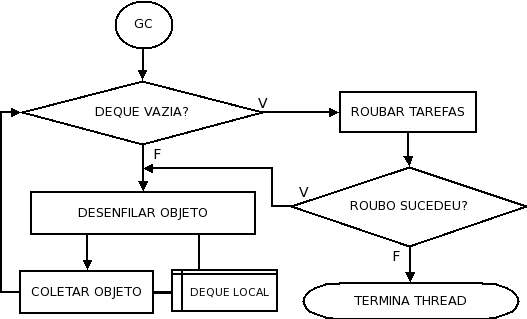
\includegraphics[width=0.8\textwidth]{images/gc_flow22.png}
\caption{Fluxograma representando a execução das {\it threads}.}
\label{fig:flow2}
\end{figure}


%\texttt{push\_bottom} e \texttt{pop\_bottom} são operações locais que, em geral, não exigem estratégias de sincronização de \textit{threads}. Sincronização é necessária apenas quando se quer retirar o último elemento da {\it deque} local ou quando uma \textit{thread} precisa roubar um elemento de outra {\it deque}.

%Nesta implementação, todas operações sobre as {\it deques} são feitas sob {\it mutexes}, ou seja, são bloqueantes. A quantidade de memória utilizada por cada {\it deque} é fixa, 

%\lstinputlisting[language=C, label=src:deque,
%								 caption=Implementação.]
%								 {codes/deque.c}



\subsection{Balanceamento dinâmico de carga} \label{sec:balanc}
Uma vez que várias \textit{threads} irão trabalhar na coleta de lixo, é importante que nenhuma delas fique sobrecarregada, enquanto outras estão desocupadas. Flood e Detlefs \cite{bib:flood:pargc} afirmam que dividir igualmente os objetos-raiz entre as \textit{threads} não evita a desproporcionalidade, pois alguns objetos-raiz podem originar grandes estruturas de dados, enquanto outros referenciam variáveis simples, como inteiros.
O balanceamento dinâmico de carga é feito utilizando a abordagem mostrada na seção anterior: cada \textit{thread} obtém uma tarefa -- referência a um objeto que deve ser coletado -- de sua {\it deque} local ou de outra {\it deque} e, durante a coleta, enfila todas as referências deste objeto em sua própria {\it deque} e assim por diante.

Como exemplo, os autores citam a aplicação deste algoritmo a uma árvore binária: uma das \textit{threads} efetuará a varredura e coleta do nodo raiz, enfilar ambos nodos filhos e desenfilar de sua {\it deque} local um dos filhos. O outro nodo filho estará disponível para ser ``roubado'' por uma outra thread. Deste modo, para uma árvore de tamanho considerável, a carga estará balanceada entre as {\it threads}.


\section{Implementação da coleta de cópia paralela} \label{sec:parcopy}
Neste projeto pretende-se paralelizar a estratégia de cópia de dois espaços, visto que esta pode apresentar resultados mais rapidamente; e também por ser aplicada em outras estratégias de coleta, como a de gerações.%TALK MORE?

Quando o sistema de execução da {\tt pFun} solicita coleta de lixo, dá-se início ao processo de distribuição dos $r$ objetos-raiz entre as $n$ {\it deques}. Após, as $n$ {\it threads} iniciam a execução da rotina mostrada no Programa \ref{src:parcol}. O primeiro passo é utilizar o argumento {\tt info} para descobrir qual das $n$ {\it deques} corresponde à {\it thread} em execução (linhas 4 e 5). A variável ponteiro {\tt task} é responsável por referenciar o objeto que deve ser coletado no corrente momento (linhas 13 e 15). A rotina {\tt par\_evacuate} da linha 16 efetua a cópia do objeto para a região inativa, retornando o novo endereço do objeto copiado.

\lstinputlisting[language=C, label=src:parcol,
								 caption=Rotina simplificada de execução das {\it threads}.]
								 {codes/par_collect.c}

A repetição das linhas 11 a 17 executa até que {\tt deq} fique sem objetos para coletar, então a linha 19 executa uma rotina de busca por algum ponteiro (objeto a ser coletado) de outra {\it deque}. Se encontrado, o novo ponteiro é armazenado em {\tt task} e enfilado na {\it deque} correspondente, e a execução do programa volta para a linha 11. No caso de {\tt steal\_some\_work()} não conseguir ``roubar'' uma tarefa, este retornará o ponteiro nulo, sinalizando que a {\it thread} corrente deve terminar sua execução.


\subsection{Cópia dos objetos vivos}
A cópia dos objetos sobreviventes para a região de destino é feita pela rotina {\tt par\_evacuate()}, de acordo com o Programa \ref{src:parevac}, onde a variável {\tt heapcell} referencia o objeto a ser copiado. Existem dois tipos de objetos: objetos apenas com dados, como valores numéricos e objetos de controle do programa, representados pelo tipo {\tt SimpleObject}; e objetos com dados e referências a outros objetos, estes podem ser listas, funções, etc., que são representados pelo tipo {\tt PointerObject}.

O primeiro passo é descobrir qual é o objeto referenciado pela variável {\tt heapcell}, para tal, basta acessar o primeiro elemento do objeto (linha 2). Em ambos casos, deve-se alocar um novo espaço correspondente ao objeto a ser coletado na região de destino: {\tt SimpleObject} usa a rotina {\tt vmsizeof()}, que calcula o tamanho do objeto na {\it heap}. Entretanto, {\tt PointerObject} deve utilizar outra rotina, {\tt objsize()}, que acrescenta o número de referências no cálculo do tamanho.

\lstinputlisting[language=C, label=src:parevac,
								 caption=Rotina simplificada de coleta paralela.]
								 {codes/par_evacuate.c}

Os testes das linhas 6 e 12 verificam se o objeto a ser coletado já foi copiado. Se for o caso, a rotina de alocação paralela (Programa \ref{src:paralloc}) retorna um ponteiro nulo, então deve-se retornar o endereço do objeto; caso contrário, deve-se copiar o conteúdo do objeto no espaço de origem para o novo endereço na região de destino (linhas 7 e 13). A operação para um {\tt SimpleObject} está completa e seu endereço é retornado na linha 8. Já para um {\tt PointerObject} deve-se posicionar {\tt pobj->pointers} no endereço de memória imediatamente posterior ao último elemento da estrutura de dados referenciada por {\tt pobj} (linha 15), então, copia-se o conteúdo de cada ponteiro para a nova posição correspondente na região de destino, colocando-os na {\it deque} local para serem coletados nos próximos instantes. Por fim, a linha 21 retorna uma referência a nova posição de memória correspondente ao objeto que acabou de ser copiado.

\subsection{\textit{Local Allocation Buffers}} \label{sec:lab}
Na coleta de lixo paralela, várias {\it threads} podem alocar objetos na região de destino ao mesmo tempo. Christine Flood e David Detlefs \cite{bib:flood:pargc} comentam que manter apenas uma variável indicativa de topo na região de destino resultaria em muitas condições de corrida, visto que pequenos objetos são alocados com muita frequência por várias {\it threads}. Para evitar o excesso de sincronizações, este projeto adotou os chamados {\it Local Allocation Buffers} (LABs), onde cada {\it thread} aloca uma porção da região de destino ({\it buffer}) com tamanho considerável, podendo alocar objetos com acesso exclusivo àquela porção, sem necessidade de sincronização. Os LABs devem ser grandes o bastante para evitar contenções por excesso de sincronização de {\it threads}, mas suficientemente pequenos para minimizar fragmentações.

Um LAB é alocado utilizando {\it mutexes}, como mostra o Programa \ref{src:LAB}. Primeiramente, o {\it mutex} correspondente ao LAB é trancado, garantindo assim, acesso exclusivo à variável compartilhada {\tt LAB\_tstop}, que referencia a posição de início do próximo LAB na {\it heap}. Após, {\tt LAB\_tstop} é copiado para uma variável auxiliar e incrementado de acordo com o indicado por {\tt size}. Ao fim, o {\it mutex} é liberado e a rotina de alocação retorna à posição de início do LAB recém alocado.

\lstinputlisting[language=C, label=src:LAB,
								 caption=Alocação de um LAB.]
								 {codes/allocLAB.c}

\subsection{Utilização da instrução CAS} \label{sec:cas}
O programa \ref{src:paralloc} mostra a rotina de alocação paralela nos LABs utilizando CAS. Nesta rotina, a variável {\tt me} identifica a {\it thread} correspondente à alocação. A linha 4 verifica se o LAB em utilização já foi preenchido e, se necessário, outro LAB é alocado. A instrução CAS é utilizada na linha 7 para evitar que um objeto, referenciado pela variável {\tt oldloc}, não seja copiado mais de uma vez. Se {\tt oldloc} já estiver na tabela de objetos copiados (variável ponteiro {\tt forwarding}), o teste da linha 8 será verdadeiro, interrompendo a alocação; caso contrário, CAS copia o valor de {\tt labtop[me]} para a tabela de objetos copiados correspondente à {\tt oldloc} e procede a alocação do espaço para este objeto no LAB (linhas 10 e 11), retornando a porção recém alocada (linha 13).


\lstinputlisting[language=C, label=src:paralloc,
								 caption=Rotina de alocação paralela.]
								 {codes/par_alloc.c}


A Figura \ref{fig:cas1} exemplifica o caso em que duas {\it threads} referenciam o mesmo objeto na região de origem (um inteiro), através de outros objetos (uma lista e uma função) já coletados. Apenas uma cópia deste inteiro pode consolidar-se. A instrução CAS é utilizada justamente para evitar que este objeto, duplamente referenciado, não seja copiado mais de uma vez. A outra referência deve ser atualizada para a nova posição do inteiro na região de destino, como mostra a Figura \ref{fig:cas2}, onde existe apenas uma cópia do objeto em questão, e tanto a lista quanto a função referenciam esta mesma cópia.

\begin{figure}[h]
\centering
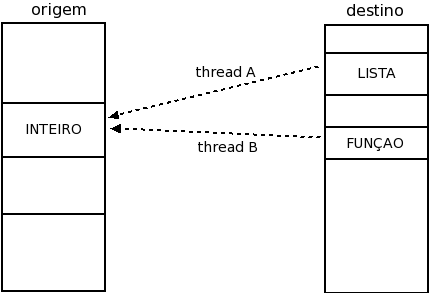
\includegraphics[width=0.6\textwidth]{images/CAS1.png}
\caption{Duas {\it threads} referenciam o mesmo objeto ainda não coletado.}
\label{fig:cas1}
\end{figure}

Se o inteiro já estiver na tabela de objetos copiados, não ocorrerá alocação, apenas atualização da referência; caso contrário, CAS insere o novo endereço do objeto na posição correspondente da tabela de objetos copiados, procedendo a alocação do espaço para este objeto no LAB.

\begin{figure}[h]
\centering
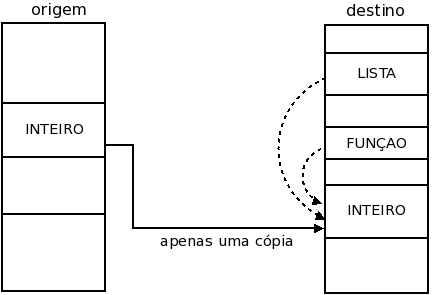
\includegraphics[width=0.6\textwidth]{images/CAS2.png}
\caption{Cópia do objeto e atualização das referêcnias utilizando CAS.}
\label{fig:cas2}
\end{figure}

%Para auxiliar no processo, mantém-se uma tabela de objetos copiados, representada pela variável ponteiro {\tt forwarding}, que é responsável por armazenar o novo endereço de um objeto da região de origem que foi copiado para a região de destino.

\chapter{Conclusões} \label{sec:finalizing}
%Conclui-se que a conclusão é importante para concluir o trabalho.
Linguagens funcionais tem sido muito utilizadas em meios acadêmicos, mas algumas delas estão cada vez mais sendo empregadas em sistemas comerciais modernos, como {\tt Erlang}, {\tt OCaml}, e {\tt Haskell}. Estas linguagens exigem que seu sistema de execução possua gerência automática de memória, de forma a facilitar a definição das construções de alto nível que a linguagem oferece.

Arquiteturas multicore estão cada vez mais populares, fazendo com que cada vez mais usuários disponham de, ao menos, dois núcleos de processamento em seus computadores pessoais. Por isso, tornam-se importante pesquisas e desenvolvimento de aplicações que façam uso desse poder computacional. %Este trabalho vem a contribuir neste aspecto: aproveitar a disponibilidade de computação -- mais núcleos de processameto disponíveis -- para melhorar o desempenho de programas escritos em {\tt pFun}.

O presente projeto apresentou uma estrutura para coleta de lixo paralela -- a coleta de cópia de dois espaços -- para uma linguagem funcional pura. Embora não tenha obtido ganhos de desempenho, o projeto contribui ao verificar as dificuldades e limites gerados pela programação {\it multi-thread} em processadores multicore. As próximas seções discutem os resultados obtidos e algumas considerações a respeito do desempenho desta implementação. % da implementação paralela da coleta de lixo. %... WHAT A MESS!

\section{Resultados obtidos}
Foram realizados testes de desempenho da máquina virtual {\tt pfun} com a coleta de lixo paralela para dois programas: {\tt pmaze} e {\tt hanoi} \cite{bib:beloni}. Nestes testes, mostrados nas Tabelas \ref{tab:res} e \ref{tab:res2}, três tempos de execução são levados em consideração: o tempo real, referente ao tempo de execução do programa; o tempo total, que é a soma dos tempos de ocupação de processadores por parte de cada programa; e o tempo aproximado de ocupação dos processadores somados nos período de realização das coletas de lixo.

Também foi verificado o desempenho da coleta de lixo sequencial, apresentada na seção \ref{sec:twospace}, que produziu melhores resultados que a coleta de lixo paralela: $14m$ para o programa {\tt pmaze} e $169m 30s$ para o programa {\tt hanoi}, sendo cerca de $1m 50s$ e $1m$ gastos com coleta de lixo, respectivamente.

\begin{table}[h]
\centering
	\begin{tabular}{c|c|c|c}
	\hline
	Processadores	& \multicolumn{3}{c}{Programa pmaze} \\
	\cline{2-4}
								& real			& total 		& coletas \\
	\hline
	2							&	18m 47s		&	24m 2s 		& 12m \\
	\hline
	4							& 20m 59s		& 43m 18s 	& 31m \\
	\hline
	6							& 22m 7s		& 64m 40s 	& 53m \\
	\hline
	8							& 24m 11s		& 96m 14s 	& 85m \\
	\hline
	\end{tabular}
\caption{Tempos de execução do programa {\tt pmaze} com coleta de lixo paralela.}
\label{tab:res}
\end{table}

\begin{table}[h]
\centering
	\begin{tabular}{c|c|c|c}
	\hline
	Processadores	& \multicolumn{3}{c}{Programa hanoi} \\
	\cline{2-4}
								& real			& total			& coletas \\
	\hline
	2							&	190m 8s		&	194m 49s 	& 21m \\
	\hline
	4							& 192m 58s	& 206m 44s 	& 31m \\
	\hline
	6							& 193m 11s	& 219m 26s 	& 48m \\
	\hline
	8							& 196m 36s	& 231m 3s 	& 63m \\
	\hline
	\end{tabular}
\caption{Tempos de execução do programa {\tt hanoi} com coleta de lixo paralela.}
\label{tab:res2}
\end{table}

Os testes apontam que, aumentando o número de processadores, o tempo real de execução é acrescido de poucos minutos, entretanto, o tempo somado de execução do programa nas CPUs tem um acréscimo considerável.

Percebe-se que os tempos de espera se agravam com o aumento do número de processadores: quanto mais processadores, mais pausas e maior o tempo de espera na coleta de lixo. Observou-se também que, ao subtrair o tempo gasto com coleta de lixo do tempo total de execução, para ambos programas, o resultado é um tempo muito próximo ao tempo de execução produzido pela coleta de cópia sequencial, ou seja, a coleta de lixo paralela está realmente gerando um gargalo. O programa {\tt pmaze} apresenta números ainda mais discrepantes, visto que este possui maior residência na {\it heap}. As próximas subseções discorrem as possíveis causas deste comportamento.

%, basta ver os resultados dos testes, o tempo do usuário é a soma dos tempos de todas as CPU!!!
%Percebe-se que um dos fatores que contribui para isto é a implementação das {\it deques}, que possui exclusão mútua em todas operações para evitar as condições de corrida, portanto, sempre que alguma {\it thread} ficar sem objetos para coletar, poderão ocorrer várias situações de exclusão mútua, que se agravam com o aumento do número de processadores: quanto mais processadores, mais pausas e maior o tempo de espera na coleta de lixo, basta ver os resultados dos testes, o tempo do usuário é a soma dos tempos de todas as CPU!!!


\subsection{Quanto aos \textit{overheads} da implementação proposta}
%Durante o desenvolvimento deste, utilizou-se a técnica de {\it overpartition} apresentada na seção \ref{sec:overp} que, apesar de balancear a carga entre as {\it threads} de maneira satisfatória, demostrou-se mais adequada para tarefas com alta granulosidade (tarefas maiores). Sabe-se que o processo de enfilar e desenfilar referências a objetos na {\it heap} ocorre com muita frequência, adicionando um {\it overhead} considerável, já que, muitas vezes, o tamanho dos objetos copiados é muito pequeno para que valham a pena tantas operações. %de enfilar e desenfilar.
Durante o desenvolvimento deste projeto, utilizou-se a técnica de {\it overpartition} apresentada na seção \ref{sec:overp}. Esta técnica efetivamente garante o balanceamento da carga entre as várias {\it threads}, entretanto, o processo de enfilar e desenfilar referências a objetos nas {\it deques} ocorre com muita frequência (Programas \ref{src:parcol} e \ref{src:parevac}), adicionando um {\it overhead} considerável, já que, muitas vezes, o tamanho dos objetos copiados é muito pequeno para que valham a pena tantas operações.

%Outro fator que pode justificar a lentidão do coletor de cópia paralela é a
A proposta original de Arora \cite{bib:arora:worksteal} é uma implementação das {\it deques} com {\it work-stealing} não bloqueante, utilizando a instrução CAS. Todavia, a implementação das {\it deques} adotada neste projeto (seção \ref{sec:worksteal}) é muito mais simples, pois está preparada para lidar com as colisões de {\it threads} usando exclusão mútua. Cada operação sobre as {\it deques} é limimtada por {\it mutexes}, desta maneira, uma situação que exigir {\it work-stealing} faz com que apenas uma {\it thread} tenha acesso à {\it deque}, bloqueando as outras {\it threads}.
%, desde o teste se a {\it deque} contém elementos até o retorno da refrência é feito sob {\it mutexes}, contribuindo para o fraco desempenho desta proposta.

Sempre que uma {\it thread (A)} tentar roubar algum elemento de outra {\it deque}, perde-se muito tempo. Primeiramente, {\it (A)} deve testar o {\it mutex} da {\it deque} vítima, que provavelmente estará na cache de outro processador, correspondente à {\it thread} dona da vítima devido a frequência de acessos, como comentado na seção \ref{sec:cache}. Se conseguir roubar o elemento, haverá um custo adicional no acesso aos elementos da {\it deque} vítima, além de trancar o acesso desta {\it deque} para qualquer outra {\it thread} que tente acessá-la, inclusive para a {\it thread} correspondente à vítima.

\subsection{Quanto às arquiteturas multicore}
As limitações impostas pelo {\it hardware} também devem ser consideradas. Mesmo que uma arquitetura disponha de vários processadores, se estes não puderem acessar a memória literalmente ao mesmo tempo, por meio de barramentos separados, o ganho de desempenho será muito prejudicado. No caso da coleta de lixo, em que a memória é constantemente acessada ({\it heap}), certamente ocorrem casos de processadores esperando por outros, além de problemas de coerência de cache apresentados na seção \ref{sec:cache}.
%Access to RAM is serialized; this and cache coherency issues causes performance to lag slightly behind the number of additional processors in the system.

\section{Continuação do trabalho}
A implementação da estrutura {\it deques} com certeza merece mais atenção, visando torná-la menos bloqueante e mais prática, seguindo a proposta de \cite{bib:arora:worksteal}, onde a instrução CAS é utilizada nos métodos {\tt pop}, em vez de exclusão mútua. % para manter a estrutura segura quanto às {\it threads}.

Também pode-se adotar a modificação efetuada por \cite{bib:flood:pargc}, em que as {\it deques} possuem um esquema para gerenciamento de {\it overflow}. Neste esquema, cada {\it deque} possui uma capacidade fixa; quando não há mais espaço, o método {\tt pop\_bottom} move uma porção dos elementos da {\it deque} correspondente para um {\it overflow set} global, liberando espaço para novas inserções. Outra possibilidade é a implementação das {\it deques} como uma lista encadeada de {\it arrays}, assim quando um array estiver lotado, um novo será alocado.

Os objetos alocados na {\it heap}, juntamente com suas referências, podem ser vistos como um conjunto de grafos. Então estudos sobre algoritmos paralelos de percurso em grafos, como em \cite{bib:bfs}, podem ser de grande valor para ajudar na melhora do desempenho da implementação.


% Bibliografia
% http://liinwww.ira.uka.de/bibliography/index.html
% um site que cataloga no formato bibtex a bibliografia em computacao
%\bibliography{nomedoarquivo.bib} (sem extensao)
%\bibliographystyle{formato.bst} (sem extensao)

\bibliography{mono}
\bibliographystyle{abnt}

% Anexos (Opcional)
%\annex 
%\chapter{Um Anexo}

%  Bla blabla blablabla bla.  Bla blabla blablabla bla.  Bla blabla blablabla
%  bla.  Bla blabla blablabla bla.  Bla blabla blablabla bla.  Bla blabla
%  blablabla bla.  Bla blabla blablabla bla.  Bla blabla blablabla bla.  Bla
%  blabla blablabla bla.  Bla blabla blablabla bla.  Bla blabla blablabla bla.
%  Bla blabla blablabla bla.  Bla blabla blablabla bla.  Bla blabla blablabla
%  bla.  Bla blabla blablabla bla.  Bla blabla blablabla bla.  Bla blabla
%  blablabla bla.  Bla blabla blablabla bla.  Bla blabla blablabla bla.  Bla
%  blabla blablabla bla.  Bla blabla blablabla bla.
\end{document}

